\documentclass{beamer}
\usepackage[utf8]{inputenc}

\usetheme{Madrid}
\usecolortheme{default}
\usepackage{amsmath,amssymb,amsfonts,amsthm}
\usepackage{txfonts}
\usepackage{tkz-euclide}
\usepackage{listings}
\usepackage{adjustbox}
\usepackage{array}
\usepackage{tabularx}
\usepackage{gvv}
\usepackage{lmodern}
\usepackage{circuitikz}
\usepackage{tikz}
\usepackage{graphicx}
\usepackage{enumitem}

\setbeamertemplate{page number in head/foot}[totalframenumber]

\usepackage{tcolorbox}
\tcbuselibrary{minted,breakable,xparse,skins}



\definecolor{bg}{gray}{0.95}
\DeclareTCBListing{mintedbox}{O{}m!O{}}{%
  breakable=true,
  listing engine=minted,
  listing only,
  minted language=#2,
  minted style=default,
  minted options={%
    linenos,
    gobble=0,
    breaklines=true,
    breakafter=,,
    fontsize=\small,
    numbersep=8pt,
    #1},
  boxsep=0pt,
  left skip=0pt,
  right skip=0pt,
  left=25pt,
  right=0pt,
  top=3pt,
  bottom=3pt,
  arc=5pt,
  leftrule=0pt,
  rightrule=0pt,
  bottomrule=2pt,
  toprule=2pt,
  colback=bg,
  colframe=orange!70,
  enhanced,
  overlay={%
    \begin{tcbclipinterior}
    \fill[orange!20!white] (frame.south west) rectangle ([xshift=20pt]frame.north west);
    \end{tcbclipinterior}},
  #3,
}
\lstset{
    language=C,
    basicstyle=\ttfamily\small,
    keywordstyle=\color{blue},
    stringstyle=\color{orange},
    commentstyle=\color{green!60!black},
    numbers=left,
    numberstyle=\tiny\color{gray},
    breaklines=true,
    showstringspaces=false,
}
%------------------------------------------------------------
%This block of code defines the information to appear in the
%Title page
\title %optional
{2.9.2}
\date{September 18, 2025}

\author 
{Shreyas Goud Burra - EE25BTECH11051}
\begin{document}

\frame{\titlepage}

\begin{frame}{Question}
    If (-5, 3) and (5, 3) are two vertices of an equilateral triangle, then the
coordinates of the third vertex, given that the origin lies inside the triangle (take $\sqrt{3}$ = 1.7), are
\end{frame}

\begin{frame}{Given Information}
    Let the two given points be represented as vectors, \textbf{A} and \textbf{B}, respectively

\begin{align}
    \textbf{A} = \myvec{-5\\3}, \textbf{B} = \myvec{5\\3}
    \label{0.1}
\end{align}

Let us assume the third point be \textbf{C}.\\
\end{frame}

\begin{frame}{Solution}
We have to first find the line equation of the line joining the points A and B.

\begin{align}
    \textbf{x} = \textbf{A} + t(\textbf{B}-\textbf{A})
    \label{0.2}
\end{align}

This gives,

\begin{align}
    \textbf{x} = \myvec{-5\\3}+t\myvec{10\\0}
    \label{0.3}
\end{align}

\end{frame}

\begin{frame}{Continuation}
We have to find the lines aligned at $60^{\circ}$ to this line at both \textbf{A} and \textbf{B}.\\
We can get this by multiplying a rotation vector to this vector, this is given by,

\begin{align}
    \textbf{V}(\theta) = \myvec{\cos\theta & -\sin\theta \\\sin\theta & \cos\theta}
    \label{0.4}
\end{align}

By multiplying this to \ref{0.3} with $\theta = \pm 60^{\circ}$, we get the lines,

\end{frame}
\begin{frame}{Continuation}
\begin{align}
    \textbf{x} = \myvec{-5\\3} + t(\textbf{V}(\pm 60^{\circ}))\myvec{1\\0}
    \label{0.5}
\end{align}

The lines we get from this equation are,

\begin{align}
    \textbf{x} = \myvec{-5\\3}+t\myvec{\frac{1}{2}\\\frac{\sqrt{3}}{2}}
    \label{0.6}
\end{align}
\end{frame}

\begin{frame}{Continuation}

\begin{align}
    \textbf{x} = \myvec{-5\\3}+t\myvec{\frac{1}{2}\\\frac{-\sqrt{3}}{2}}
    \label{0.7}
\end{align}

By doing the same thing taking point B,

\begin{align}
    \textbf{x} = \myvec{5\\3}+t\myvec{\frac{1}{2}\\\frac{\sqrt{3}}{2}}
    \label{0.8}
\end{align}

\end{frame}
\begin{frame}{Continuation}
\begin{align}
    \textbf{x} = \myvec{5\\3}+t\myvec{\frac{1}{2}\\\frac{-\sqrt{3}}{2}}
    \label{0.9}
\end{align}

We can get two possible points that fit the given conditions for an equilateral triangle, let us assume these to be \textbf{C1} and \textbf{C2}\\

We can get \textbf{C1} by finding the point of intersection of \ref{0.6} and \ref{0.9}
\begin{align}
    \myvec{-5\\3} + t\myvec{\frac{1}{2}\\\frac{\sqrt{3}}{2}} = \myvec{5\\3} +t\myvec{\frac{1}{2}\\\frac{-\sqrt{3}}{2}}
    \label{0.10}
\end{align}
\end{frame}
\begin{frame}{Final Answer}
On further solving, we get the point to be,
\begin{align}
    \textbf{C1} = \myvec{0\\3+5\sqrt{3}} = \myvec{0\\11.5}
    \label{0.11}
\end{align}

Similarly, on solving for the other two lines, \ref{0.7} and \ref{0.8}, we get,
\begin{align}
    \textbf{C2} = \myvec{0\\3-5\sqrt{3}} = \myvec{0\\-5.5}
    \label{0.12}
\end{align}
\end{frame}

\begin{frame}[fragile]
\frametitle{C code}
\begin{lstlisting}

#include<stdio.h>
#include<math.h>

double norm(double *A, int m){
	double norm = 0;
	for(int i=0; i<m; i++){
		norm += A[i]*A[i];
	}
	norm = sqrt(norm);
	return norm;
}

\end{lstlisting}
\end{frame}

\begin{frame}[fragile]
\frametitle{Python code}
\begin{lstlisting}
import matplotlib.pyplot as plt
import numpy as np
import ctypes
import os
import sys

norm = ctypes.CDLL('./norm.so')
norm.norm.argtypes = [
        ctypes.POINTER(ctypes.c_double),
        ctypes.c_int
]

\end{lstlisting}
\end{frame}

\begin{frame}[fragile]
\frametitle{Python code}
\begin{lstlisting}

norm.norm.restype = ctypes.c_double

A=np.array([-5, 3], dtype=np.float64)
B=np.array([5, 3], dtype=np.float64)
m=len(A)

D=B-A

fig, ax=plt.subplots()

\end{lstlisting}
\end{frame}

\begin{frame}[fragile]
\frametitle{Python code}
\begin{lstlisting}

norm = norm.norm(
        D.ctypes.data_as(ctypes.POINTER(ctypes.c_double)),
        m
)

t=(1.7/2)*norm

C1=np.array([0, 3+t], dtype=np.float64)
C2=np.array([0, 3-t], dtype=np.float64)

\end{lstlisting}
\end{frame}

\begin{frame}[fragile]
\frametitle{Python code}
\begin{lstlisting}

def line_gen_num(A,B,num):
  dim = A.shape[0]
  x_AB = np.zeros((dim,num))
  lam_1 = np.linspace(0,1,num)
  for i in range(num):
    temp1 = A + lam_1[i]*(B-A)
    x_AB[:,i]= temp1.T
  return x_AB

\end{lstlisting}
\end{frame}

\begin{frame}[fragile]
\frametitle{Python code}
\begin{lstlisting}

x_AB = line_gen_num(A, B, 20)
x_BC1 = line_gen_num(C1, B, 20)
x_BC2 = line_gen_num(C2, B, 20)
x_AC1 = line_gen_num(A, C1, 20)
x_AC2 = line_gen_num(A, C2, 20)

\end{lstlisting}
\end{frame}

\begin{frame}[fragile]
\frametitle{Python code}
\begin{lstlisting}

plt.grid()
plt.title('2.9.2')
plt.plot(x_AB[0, :], x_AB[1, :], 'r--', label='Line from A to B')
plt.plot(x_BC1[0, :], x_BC1[1, :], 'r--') 
plt.plot(x_BC2[0, :], x_BC2[1, :], 'r--') 
plt.plot(x_AC1[0, :], x_AC1[1, :], 'r--') 
plt.plot(x_AC2[0, :], x_AC2[1, :], 'r--') 

\end{lstlisting}
\end{frame}

\begin{frame}[fragile]
\frametitle{Python code}
\begin{lstlisting}

plt.plot(A[0], A[1], 'go', label='Point A')  
plt.annotate('(-5,3)', xy=(A[0],A[1]), fontsize=12)
plt.plot(B[0], B[1], 'go', label='Point B')  
plt.annotate('(5,3)', xy=(B[0],B[1]), fontsize=12)
plt.plot(C1[0], C1[1], 'bo', label='Point C1')  
plt.annotate('(0,11.5)', xy=(C1[0],C1[1]), fontsize=12)
plt.plot(C2[0], C2[1], 'bo', label='Point C2')  
plt.annotate('(5,-5.5)', xy=(C2[0],C2[1]), fontsize=12)

\end{lstlisting}
\end{frame}

\begin{frame}[fragile]
\frametitle{Python code}
\begin{lstlisting}

for axis in ['bottom', 'left']:
    ax.spines[axis].set_color('black')
    ax.spines[axis].set_linewidth(2)

\end{lstlisting}
\end{frame}

\begin{frame}[fragile]
\frametitle{Python code}
\begin{lstlisting}

plt.legend()
plt.xlabel('X-axis')
plt.ylabel('Y-axis')
plt.axis('equal')
plt.savefig('/home/shreyas/GVV_Assignments/matgeo/2.9.2/figs/fig1.png')

plt.show()
\end{lstlisting}
\end{frame}

\begin{figure}[H]
    \centering
    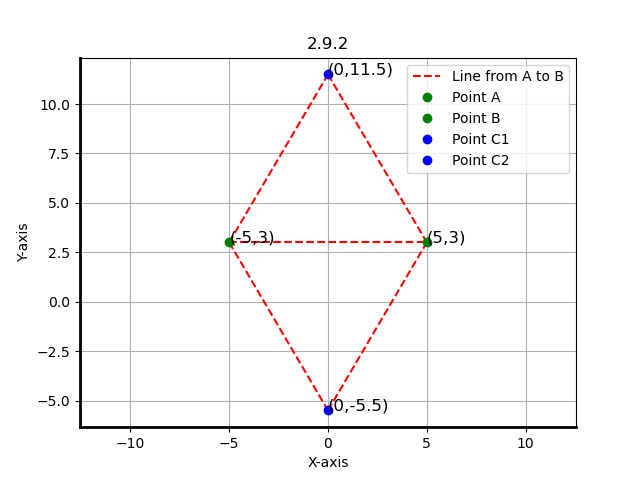
\includegraphics[width=0.8\columnwidth]{figs/fig1.png}
    \caption{2D Plot}
    \label{3D Plot}
\end{figure}
\end{document}


\end{document}
